In our study, we introduce a detailed mathematical model designed to capture the behavior of bacterial populations,
including both non-resistant and resistant strains, along with their interactions with immune cells responsible for host defense, all
within the context of antibiotic presence. Our model is built upon several key assumptions, including considerations for bacterial reproduction and death rates, the transfer of antibiotic resistance genes between bacterial strains, the impact of the antibiotic itself,
and the response of the immune system. This complex interplay is described by a system of differential equations, which outlines
the dynamic relationships between these variables and processes:

\begin{equation}
	\begin{cases}
		\dot{A}(t)  =  \Lambda - \mu A, \\
		\dot{S}(t)  =  \eta_s\left(1 - \frac{S+R}{K}\right)S - \bar{\alpha}AS - \beta\frac{SR}{N} - \Gamma SP, \\
		\dot{R}(t)  =  \eta_r\left(1 - \frac{S+R}{K}\right)R + \beta\frac{SR}{N} - \Gamma RP, \\
		\dot{P}(t)  =  \Phi(N)P\left(1 - \frac{P}{P_{\max}}\right) - \Psi(N)P, \\
	\end{cases}
\end{equation}
where $S$ represents the population of Non-Antibiotic Resistant Bacteria (NARB), $R$ stands for the population of Antibiotic Resistant
Bacteria (ARB), $P$ denotes the population of immune cells and $A$ indicates the concentration of antibiotic.

\begin{figure}
	\centering
	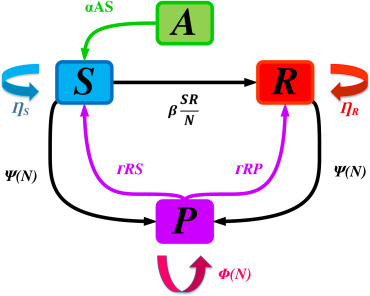
\includegraphics[width=0.6\textwidth]{1-s2.0-S1007570424005975-gr1.jpg}
	\caption{Schematic Diagram}
\end{figure}

In biological systems, the proliferation of ARB is frequently reported to exhibit a slower rate compared to NARB, owing to
a multitude of underlying reasons. These factors may include the metabolic costs associated with maintaining resistance
mechanisms, alterations in cellular physiology resulting from genetic mutations, and potential trade-offs between resistance and
other cellular functions. This phenomenon is significant as it impacts the overall dynamics of bacterial populations within ecosystems
and during infection processes. In our model, we incorporate a logistic growth terms characterized by growth rates $\eta_s$ for NARB and
$\eta_r$ for ARB, with $\eta_s > \eta_r$ , alongside a shared carrying capacity $K$.

Here, we look at how a resistance plasmid helps antibiotic-resistant genes move from bacteria types that are already resistant
to those that are not (susceptible strains). This plasmid serves as a means for the transfer of antibiotic resistance determinants
between bacteria. Biologically, this transfer is analogously perceived as analogous to the contagion dynamics observed in disease
transmission: a resistant bacterium (acting as the donor) encounters a non-resistant bacterium (the recipient), and the likelihood is
that both bacteria acquire resistance traits subsequent to the interaction. In this case, we employ the term: $\beta\frac{SR}{N}$.

The terms $\Gamma SP$ and $\Gamma RP$ describe the elimination of (NARB) and (ARB) by the immune cells. The final equation is
supported by the observed relationship between the potency of the immune response and the concentration of bacteria. Specifically,
a minor infection initiates an immune reaction, while a major infection dampens the immune response, either through the death of
immune cells or by impeding the proliferation of immune cells. $P_max$ is the maximum number of immune cells and the functions
$\Phi(N)$ and $\Psi(N)$ are supposed to be positive and belonging to $\mathrm{C}^1(\mathbb{R}_+)$.

Ultimately, the antibiotic is administered at a rate denoted by $\lambda$ and absorbed at a rate represented by $\mu$.

This model system has 9 parameters in all, which makes mathematical analysis complicated. We are going to review the
following transformation of variables:
\[ 
\begin{array}{ccccc}
	a = \frac{A}{\Lambda/\mu},\hspace{2mm} s = \frac{S}{K},\hspace{2mm} r = \frac{R}{K},\hspace{2mm} p = \frac{P}{P_{\max}},
	\hspace{2mm}
	\alpha = \frac{\bar{\alpha}A}{\mu},\hspace{2mm} \\ \gamma = \Gamma P_{\max},
	\hspace{2mm} n = s + r
\end{array}
\]

With the scaling, system (1) takes the form

\begin{equation}
	\begin{cases}
	\dot{a}(t)  =  \mu(1 - a)  \\
	\dot{s}(t)  =  \eta_s(1 - n)s - \alpha as - \beta \frac{sr}{n} - \gamma sp \\
	\dot{r}(t)  =  \eta_r(1 - n)r + \beta \frac{sr}{n} - \gamma rp \\
	\dot{p}(t)  =  \phi(n)p(1 - p) - \psi(n)p \\
	\end{cases}
\end{equation}
where
\[
\phi(n) = \Phi(Kn)
\]
and
\[
\psi(n) = \Psi(Kn).
\]

